
% v2-acmsmall-sample.tex, dated March 6 2012
% This is a sample file for ACM small trim journals
%
% Compilation using 'acmsmall.cls' - version 1.3 (March 2012), Aptara Inc.
% (c) 2010 Association for Computing Machinery (ACM)
%
% Questions/Suggestions/Feedback should be addressed to => "acmtexsupport@aptaracorp.com".
% Users can also go through the FAQs available on the journal's submission webpage.
%
% Steps to compile: latex, bibtex, latex latex
%
% For tracking purposes => this is v1.3 - March 2012
\documentclass[prodmode,acmtecs]{acmsmall} % Aptara syntax
\usepackage[spanish,polish]{babel}
\usepackage[T1]{fontenc}
\usepackage{fancyvrb}
\usepackage{graphicx,hyperref}
\newcommand\cutout[1]{}


\usepackage[table]{xcolor}
\usepackage[utf8]{inputenc}
\usepackage[parfill]{parskip}
\usepackage{tabulary}
\PassOptionsToPackage{hyphens}{url}
\usepackage{hyperref}    
\usepackage[capitalize]{cleveref}


% Metadata Information
% !!! TODO: SET THESE VALUES !!!
\acmVolume{0}
\acmNumber{0}
\acmArticle{CFP}
\acmYear{0}
\acmMonth{0}

\newcounter{colstart}
\setcounter{page}{4}

\RecustomVerbatimCommand{\VerbatimInput}{VerbatimInput}%
{
%fontsize=\footnotesize,
fontfamily=\rmdefault
}


\newcommand{\UnderscoreCommands}{%\do\verbatiminput%
\do\citeNP \do\citeA \do\citeANP \do\citeN \do\shortcite%
\do\shortciteNP \do\shortciteA \do\shortciteANP \do\shortciteN%
\do\citeyear \do\citeyearNP%
}

\usepackage[strings]{underscore}



% Document starts
\begin{document}


\setcounter{colstart}{\thepage}

\acmArticle{CFP}
\title{\huge\sc SIGLOG Monthly 230}
\author{DAVID PURSER\affil{University of Warsaw, Poland}
\vspace*{-2.6cm}\begin{flushright}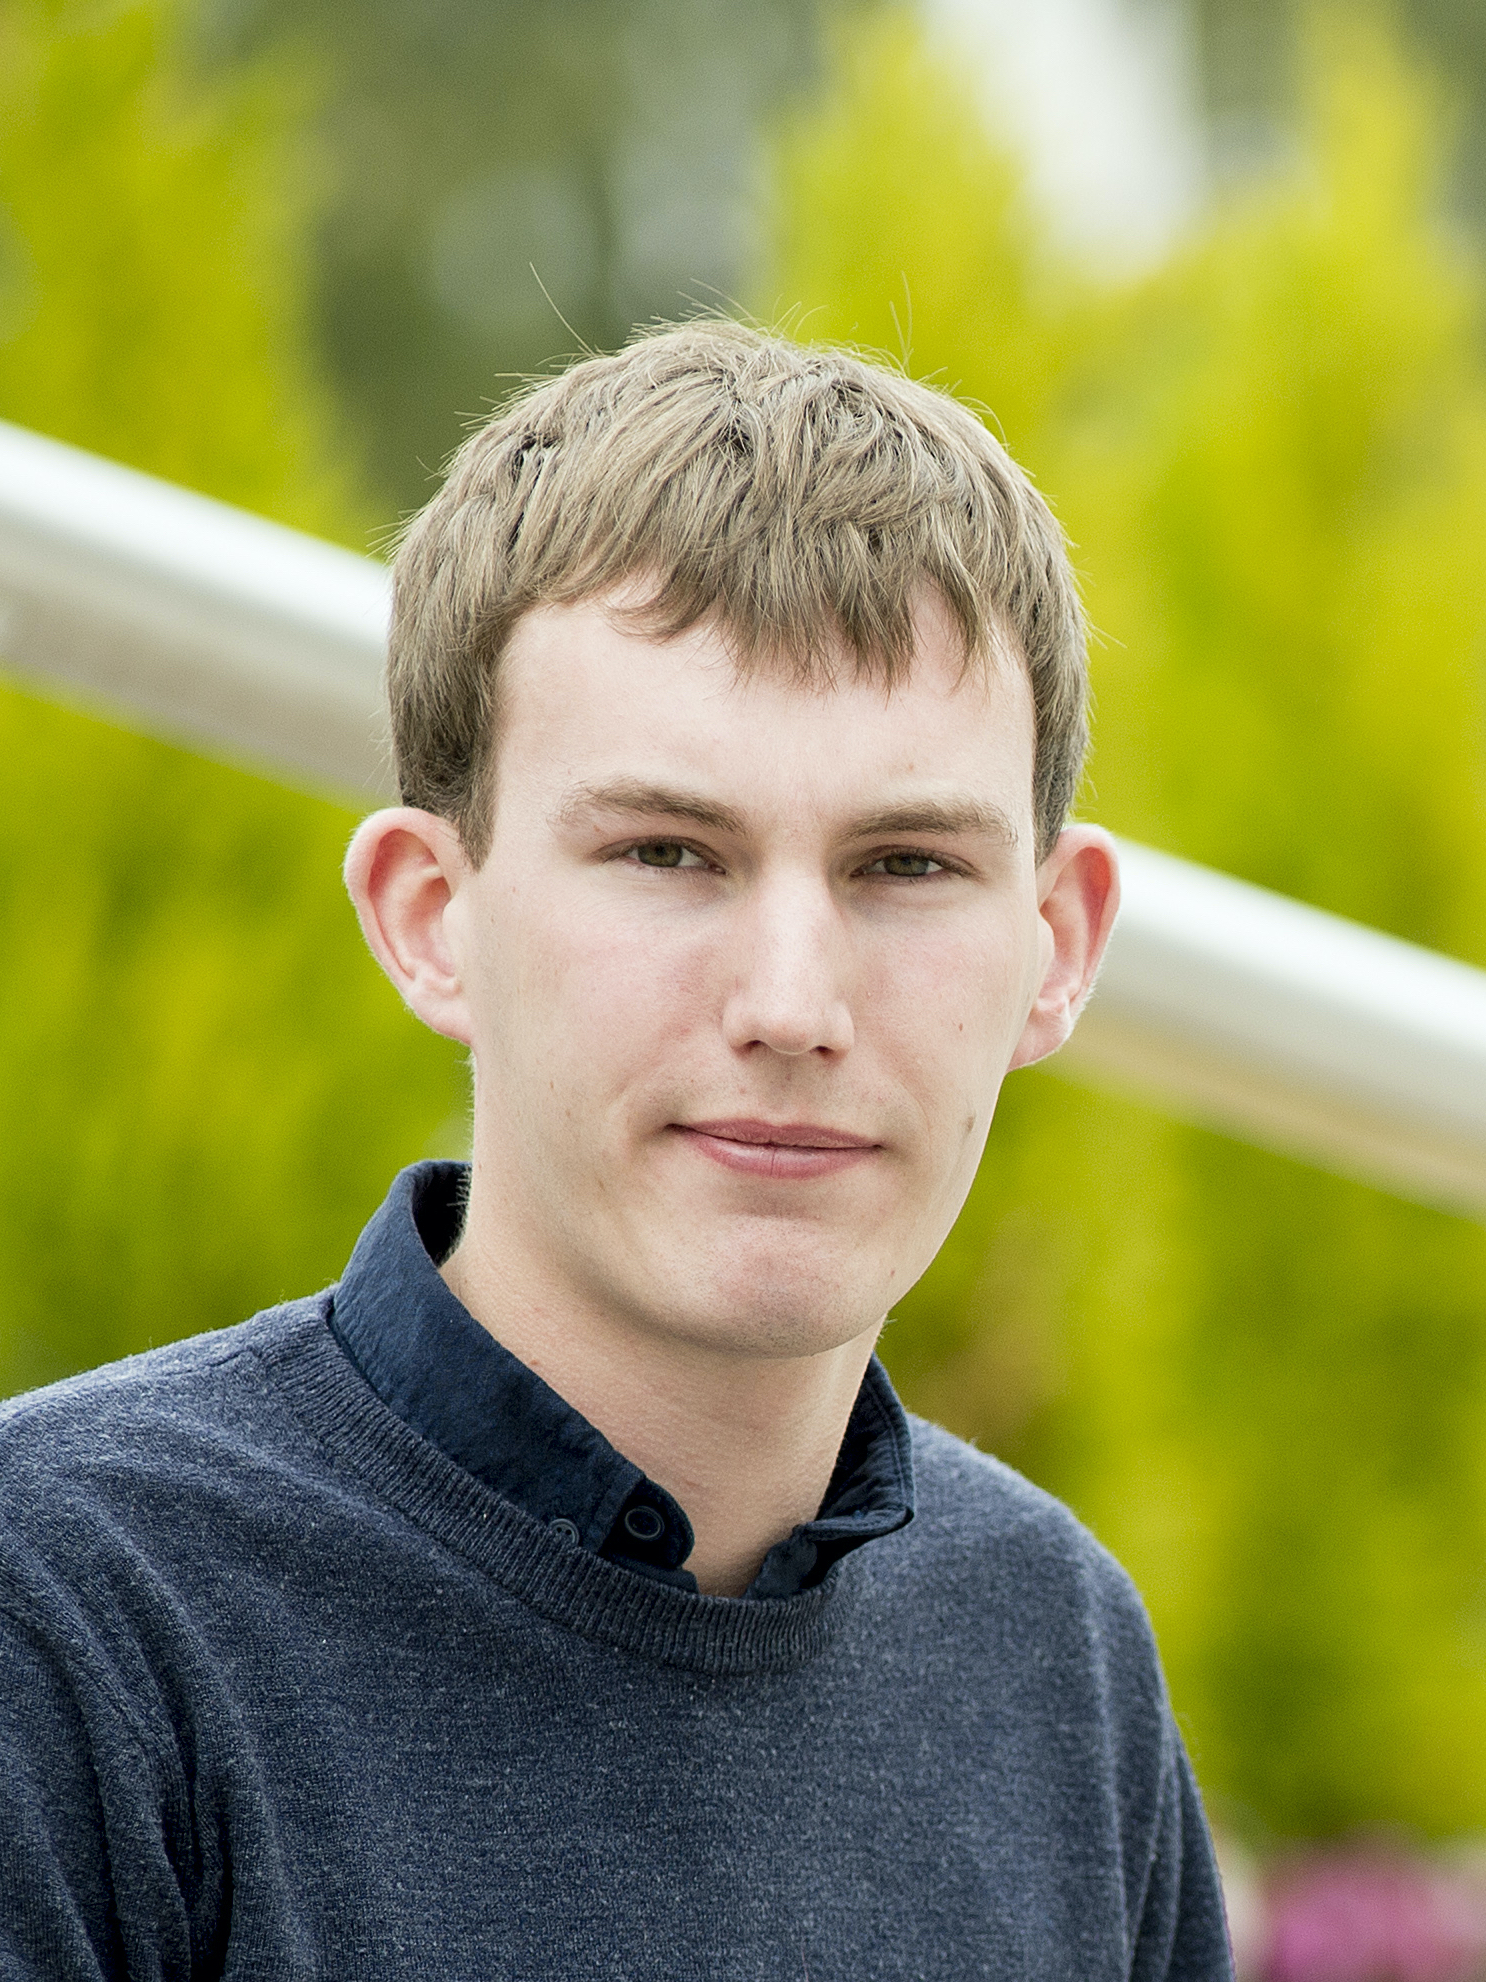
\includegraphics[width=30mm]{dp}\end{flushright}
}

\maketitlee

\href{https://lics.siglog.org/newsletters/}{Past Issues}
 - 
\href{https://lics.siglog.org/newsletters/inst.html}{How to submit an announcement}
\section{Table of Content}\begin{itemize}\item DEADLINES (\cref{deadlines}) 
 
\item SIGLOG MATTERS 
 
\begin{itemize}\item 2022 ALONZO CHURCH AWARD ANNOUNCEMENT (\cref{2022ALONZOCHURCHAWARDANNOUNCEMENT})
\item LICS 2023 (\cref{LICS2023})
\end{itemize} 
\item CALLS 
 
\begin{itemize}\item 2022 Victor Lesser Distinguished Dissertation Award (CALL FOR NOMINATIONS) (\cref{2022VictorLesserDistinguishedDissertationAward})
\item TYPES 2022 (CALL FOR POST-PROCEEDING PAPERS) (\cref{TYPES2022})
\end{itemize} 
\item JOB ANNOUNCEMENTS 
 
\begin{itemize}\item Four faculty positions in CS at Oxford (\cref{FourfacultypositionsinCSatOxford})
\end{itemize} 
\end{itemize}\section{Deadlines}\label{deadlines}\rowcolors{1}{white}{gray!25}\begin{tabulary}{\linewidth}{LL}FSEN 23:  & Oct 07, 2022 (Abstract), Oct 14, 2022 (Paper) \\
Lecturer/Senior Lecturer at UNSW, Sydney:  & Oct 12, 2022 (Formal Methods and Logic in Computer Science Job Closing) \\
ETAPS 2023:  & Oct 13, 2022 (Paper) \\
2022 Victor Lesser Distinguished Dissertation Award:  & Oct 15, 2022 (Submission deadline) \\
TYPES 2022:  & Oct 31, 2022 (Abstract), Nov 30, 2022 (Paper) \\
PODS 2023:  & Nov 28, 2022 (Second cycle abstract), Dec 05, 2022 (Full paper) \\
Oxford Faculty Positions:  & Dec 14, 2022 (noon) \\
LICS 2023:  & Jan 18, 2023 (Titles and Short Abstracts Due), Jan 23, 2023 (Full Papers Due) \\
\end{tabulary}
\section{2022 ALONZO CHURCH AWARD ANNOUNCEMENT}\label{2022ALONZOCHURCHAWARDANNOUNCEMENT}ANNOUNCEMENT 

\begin{itemize}\item  The ACM Special Interest Group on Logic (SIGLOG), the European Association for Theoretical Computer Science (EATCS), the European Association for Computer Science Logic (EACSL), and the Kurt Goedel Society (KGS) are pleased to announce that  
 
\begin{itemize}\item  Dexter Kozen
\end{itemize} 
  has been selected as the winner of the  
 
\begin{itemize}\item  2022 Alonzo Church Award for Outstanding Contributions to Logic and Computation
\end{itemize} 
  for his fundamental work on developing the theory and applications of Kleene Algebra with Tests, an equational system for reasoning about iterative programs, published in: 
 
  Kleene Algebra with Tests. ACM Transactions on Programming Languages and Systems 19(3): 427-443 (1997). 
 
\item  THE CONTRIBUTION 
 
  This work on Kleene Algebra with Tests (KAT) is one of the high points among remarkable contributions of Dexter Kozen to logics of programs. It is a culmination of a series of articles by Dexter Kozen that define and apply Kleene Algebra with Tests (KAT), an equational system that combines Kleene Algebra (the algebra of regular expressions) with Boolean Algebra (the tests). Together, the terms of the two algebras are capable of representing while programs, and their combined equational theory is capable of proving a wide range of important properties of programs. Although reasoning in KAT under arbitrary commuting conditions is undecidable, Kozen observes that when the commuting conditions are limited to including tests, it is decidable and in PSPACE. He illustrates the power of KAT with these decidable commuting conditions by proving a well-known folk theorem: Every while program can be simulated by a program with just one loop. KAT has been successfully applied to a variety of problems over the past 25 years, including modeling and reasoning about packet-switched networks. 
 
\item  The 2022 Church Award was selected by a jury consisting of Thomas Colcombet, Mariangiola Dezani, Javier Esparza, Radha Jagadeesan (chair), and Igor Walukiewicz. 
 
\end{itemize}\section{LICS 2023: The 38th Annual ACM/IEEE Symposium on Logic in Computer Science}\label{LICS2023} Boston, USA \\ 
 June 26-29, 2023 with workshops June 24-25.\\ 
CALL FOR PAPERS 

\begin{itemize}\item  The LICS Symposium is an annual international forum on theoretical and practical topics in computer science that relate to logic, broadly construed. We invite submissions on topics that fit under that rubric. Suggested, but not exclusive, topics of interest include: 
 
\begin{itemize}\item  automata theory, automated deduction, categorical models and logics, concurrency and distributed computation, constraint programming, constructive mathematics, database theory, decision procedures, description logics, domain theory, finite model theory, formal aspects of program analysis, formal methods, foundations of computability, foundations of probabilistic, real-time and hybrid systems, games and logic, higher-order logic, knowledge representation and reasoning, lambda and combinatory calculi, linear logic, logic programming, logical aspects of AI, logical aspects of bioinformatics, logical aspects of computational complexity, logical aspects of quantum computation, logical frameworks, logics of programs, modal and temporal logics, model checking, process calculi, programming language semantics, proof theory, reasoning about security and privacy, rewriting, type systems, type theory, and verification.
\end{itemize} 
\item  INSTRUCTIONS TO AUTHORS 
 
  Authors are required to submit a paper title and a short abstract of about 100 words in advance of submitting the full paper. The exact deadline time on these dates is given by anywhere on earth (AoE). 
 
\rowcolors{1}{white}{gray!25}\begin{tabulary}{\linewidth}{LL}Titles and Short Abstracts Due:  & Jan 18, 2023 \\
Full Papers Due:  & Jan 23, 2023 \\
Author Response Period:  & Mar 15-19, 2023 \\
Author Notification:  & Apr 05, 2023 \\
Conference:  & Jun 26-29, 2023 \\
\end{tabulary}
 
  Submission deadlines are firm; late submissions will not be considered. 
 
  Please see the full call for further instructions including formatting details, double-blind requirements, submission via EasyChair and other rules: \href{https://lics.siglog.org/lics23/cfp.php}{https://lics.siglog.org/lics23/cfp.php} 
 
\item  KLEENE AWARD, DISTINGUISHED PAPERS AND SPECIAL ISSUES 
 
\begin{itemize}\item  An award in honor of the late Stephen C. Kleene will be given for the best student paper(s), as judged by the program committee.
\item  Around 10% of accepted papers will be selected as distinguished papers. These are papers that, in the view of the LICS program committee, make exceptionally strong contribution to the field and should be read by a broad audience due their relevance, originality, significance and clarity.
\item  Full versions of up to three accepted papers, to be selected by the program committee, will be invited for submission to the Journal of the ACM. Additional selected papers will be invited to a special issue of Logical Methods in Computer Science.
\end{itemize} 
\end{itemize}\section{2022 Victor Lesser Distinguished Dissertation Award}\label{2022VictorLesserDistinguishedDissertationAward}CALL FOR NOMINATIONS 

\begin{itemize}\item  IFAAMAS, the International Foundation for Autonomous Agents and Multiagent Systems is pleased to announce the call for 2022 Victor Lesser Distinguished Dissertation Award.  
 
  This award is named after Professor Victor Lesser, a long-standing member of the AAMAS community who has supervised a large number of outstanding PhD students in the area. It is awarded for dissertations written as part of a PhD defended in the specified period, nominated by the supervisor (with supporting references), which show originality, significance and impact, and are supported by high quality publications. 
 
  Nominations are invited for the award which is sponsored by IFAAMAS and will be presented at AAMAS-2023. 
 
  Eligible doctoral dissertations are those defended between November 1, 2021 and October 1, 2022 in the area of Autonomous Agents or Multiagent Systems. 
 
  This award includes a certificate and a 1500 EUR payment. 
 
\item  IMPORTANT DATES  
 
Submission deadline: Oct 15, 2022 
 
\item  SELECTION PROCEDURE 
 
  The selection of the dissertation will be based on the originality, significance, and impact of the work. Evidence of such impact include publications at highly selective conferences and journals in the field, with due importance given to the AAMAS conference series and JAAMAS. Research output that resulted primarily from the student's initiative will be considered more favourably.  
 
  The selection committee will be the final arbiter in the decision process. The selection committee might also decide to consult external assessors and reserves the right to not award the prize if the nominations do not meet the expected quality level. 
 
  The dissertation must be nominated by the thesis supervisor and must be supported by the following documents, all should be delivered via the link below by Oct 15th, 2022: 
 
\begin{itemize}\item  A link to a PDF file of the dissertation. If the dissertation is not written in English, the nomination must include an accessible link to a substantial manuscript in English, with the nominee as the first author, published in a peer-reviewed journal or conference.
\item  A PDF that contains a list of publications that have arisen from the dissertation, with links to the published papers.
\item   A recommendation from the dissertation supervisor, on departmental letterhead, nominating the dissertation for the IFAAMAS-22 Victor Lesser Distinguished Dissertation Award. The recommendation should explain the contribution of the dissertation to the field of autonomous agents and multiagent systems, argue the merit and possible future impact of the work, and highlight, where relevant, how the work resulted from the initiative of the student. Finally, this document should certify the eligibility of the PhD by asserting that the PhD was defended successfully between November 1, 2021 and October 1, 2022.
\item  The names, email addresses, and affiliations of at least one and at most three referees, familiar with the research of the candidate and experts in the pertinent research area, who will directly email their recommendations for the candidate to the chair of the selection committee (Paolo Turrini, p.turrini@warwick.ac.uk). A reference letter should be no more than 500 words in length and should be on official letterhead, signed and emailed as a PDF file.
\end{itemize} 
  Note: it is the responsibility of the dissertation supervisor to contact the referees and ensure that letters (max 500 words, signed, and on letterhead) are submitted by the deadline. 
 
  Though the nomination is to be submitted by the nominee's dissertation supervisor, it is required that the nominee has consented that the dissertation be considered for this award and, if selected for the award, commits to attend the AAMAS-2023 conference, where they will receive the award and will give a presentation in a special session of the conference on the work contained in the dissertation. The cost of attending the conference is not covered by the award. 
 
\item  SUBMISSION LINK  
 
  \href{https://docs.google.com/forms/d/e/1FAIpQLSd7bU9lEkZAw9j73B4hoYghgsQmd74iDlheLvd4n4dCyN51Ng/viewform}{https://docs.google.com/forms/d/e/1FAIpQLSd7bU9lEkZAw9j73B4hoYghgsQmd74iDlheLvd4n4dCyN51Ng/viewform} 
 
\item  For questions, please contact the chair of the selection committee, Paolo Turrini (p.turrini@warwick.ac.uk). 
 
\end{itemize}\section{TYPES 2022: International Conference on Types for Proofs and Programs}\label{TYPES2022}  \href{https://types22.inria.fr/}{https://types22.inria.fr/}\\ 
CALL FOR POST-PROCEEDING PAPERS 

  TYPES is a major forum for the presentation of research on all aspects of type theory and its applications. TYPES 2022 was held from 20 to 25 June at LS2N, University of Nantes, France. The post-proceedings volume will be published in LIPIcs, Leibniz International Proceedings in Informatics, an open-access series of conference.\\ 
\begin{itemize}\item  SUBMISSION GUIDELINES 
 
  Submission is open to everyone, also to those who did not participate in the TYPES 2022 conference. We welcome high-quality descriptions of original work, as well as position papers, overview papers, and system descriptions. Submissions should be written in English, and being original, i.e. neither previously published, nor simultaneously submitted to a journal or a conference. 
 
\begin{itemize}\item  Papers have to be formatted with the current LIPIcs style and adhere to the style requirements of LIPIcs. 
\item  The upper limit for the length of submissions is 20 pages, excluding bibliography (but including title and appendices). 
\item  Papers have to be submitted as PDF. A link to the submission system will be made available on \href{https://types22.inria.fr/}{https://types22.inria.fr/}. 
\item  Authors have the option to attach to their submission a zip or tgz file containing code (formalised proofs or programs), but reviewers are not obliged to take the attachments into account and they will not be published.
\end{itemize} 
\item  DEADLINES (AoE)  
 
\rowcolors{1}{white}{gray!25}\begin{tabulary}{\linewidth}{LL}Abstract submission:  & Oct 31, 2022 \\
Paper submission:  & Nov 30, 2022 \\
Author notification:  & Mar 31, 2022 \\
\end{tabulary}
 
\item  LIST OF TOPICS 
 
  The scope of the post-proceedings is the same as the scope of the conference: the theory and practice of type theory. In particular, we welcome submissions on the following topics: 
 
\begin{itemize}\item  Foundations of type theory; 
\item  Applications of type theory (e.g. linguistics or concurrency); 
\item  Constructive mathematics; 
\item  Dependently typed programming; 
\item  Industrial uses of type theory technology; 
\item  Meta-theoretic studies of type systems; 
\item  Proof assistants and proof technology; 
\item  Automation in computer-assisted reasoning; 
\item  Links between type theory and functional programming; 
\item  Formalising mathematics using type theory; 
\item  Homotopy type theory and univalent mathematics. 
\end{itemize} 
\end{itemize}\section{Four faculty positions in CS at Oxford}\label{FourfacultypositionsinCSatOxford}JOB ANNOUNCEMENT 

\begin{itemize}\item  The University of Oxford Computer Science Department is hiring four new faculty 
 
\begin{itemize}\item  The positions are open to all areas of computer science.
\item  The closing date is 12 noon on 14 December 2022. 
\item  For more information, see \href{https://www.cs.ox.ac.uk/aboutus/vacancies/vacancy-faculty-hiring.html}{https://www.cs.ox.ac.uk/aboutus/vacancies/vacancy-faculty-hiring.html}
\end{itemize} 
\end{itemize}


To the \href{http://siglog.org/}{SIGLOG} or \href{https://lics.siglog.org}{LICS} website\end{document}